%%%%%%%%%%%%%%%%%%%%%%%%%%%%%%%%%%%%%%%%%%%%%%%%%%%%%%%%%%%%
% TESTS : PLANIFICATION QBF
%%%%%%%%%%%%%%%%%%%%%%%%%%%%%
\subsection{Planification : codages compacts avec QBF}

% vérifier le comptage des clauses sur quelques exemplesTODO: vérifier le comptage des clauses (avec touist). Comparaison de la taille des codages SAT/QBF en faveur de QBF ?
%\mael{Mael: j'ai viré la référence à TouIST pour le blind review}
%To compare these three encodings on a same basis we used our the translator TouIST\footnote{\url{https://www.irit.fr/touist}}. It can use several QBF solvers, as for example RAReQS~\cite{DBLP:conf/sat/JanotaKMC12}, DepQBF~\cite{DBLP:conf/cade/LonsingE17}, and Qute~\cite{Peitl2017} but the results are only given for the solver RAReQS based on recursively using counterexample abstraction refinement (CEGAR) \cite{DBLP:journals/jacm/ClarkeGJLV03} because it performed better than others.
Pour comparer ces trois codages sur une même base, nous avons utilisé notre traducteur TouIST\footnote{\url{https://www.irit.fr/touist}} \cite{DBLP:journals/corr/SlimaneCGHLMV15} qui peut faire appel à différents solveurs.
Nous avons utilisé tous les benchmarks IPC STRIPS disponibles (1 à 8, excepté le 7$^{\text{ème}}$ que les auteurs ne nous ont pas transmis) sur un CPU Intel\textregistered\ Xeon\textregistered\ E7-8890 v4 @ 2.20GHz, 512 Go de RAM. Les domaines testés incluent Gripper, Logistics, Mystery, Blocks, Elevator, Depots, DriverLog, ZenoTravel, FreeCell, Airport, Pipesworld-NoTankage, Pipesworld-Tankage, PSR, Satellite, OpenStacks, Pathways, Rovers, Storage, TPP, Trucks, ChildSnack, Hiking, VisitAll et le domaine non-IPC Ferry.

Nous avons essayé de considérer autant de solveurs QBF que possible en utilisant QBFEval 2017 comme référence. Qute (version du 09/07/2017, basé sur l'apprentissage par dépendance QCDCL) et CaQE (version du 08/07/2017, basé sur l'abstraction clausale de CEGAR) n'étaient pas capables de donner une valuation pour le quantificateur existentiel externe. AIGSolve et Qell n'étaient pas disponibles au téléchargement. GhostQ n'a pas été utilisé (mais nous aurions dû l'inclure). DepQBF (version 6.03 du 02/08/2017, basé sur la \enquote{Q-résolution généralisée}, décrite dans \cite{DBLP:conf/cade/LonsingE17}) et RAReQS (version 1.1 du 2013-05-07, basé sur une approche CEGAR, détaillée dans \cite{DBLP:conf/sat/JanotaKMC12}) étaient les seuls solveurs restants. RAReQS était toujours deux fois plus rapide que DepQBF, nous avons donc rejeté DepQBF et seulement conservé les résultats pour RAReQS. Enfin, nous n'avons appliqué aucun préprocesseur QBF (par exemple, Bloqqer).


\begin{figure}[ht!] \centering
\begin{center} 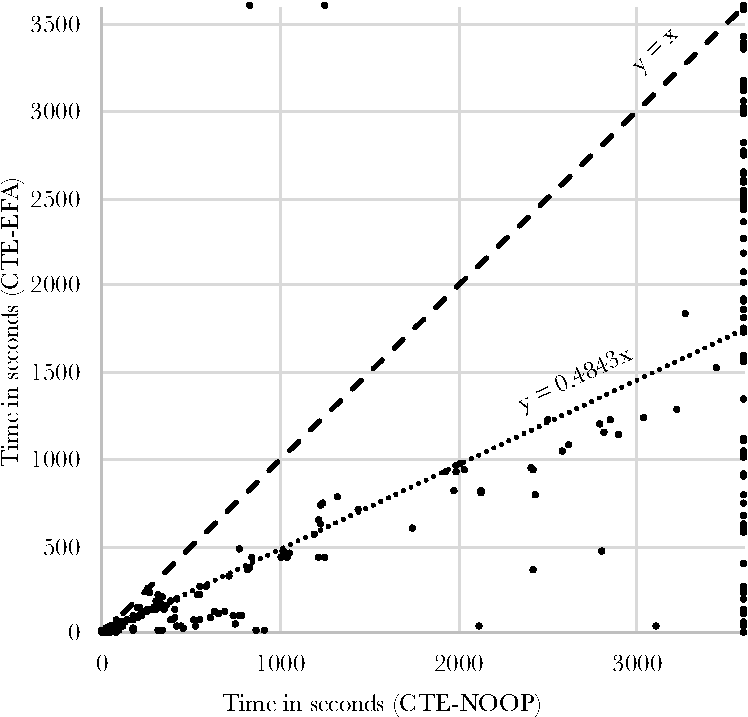
\includegraphics[width=.48\textwidth]{figures/time-plansat-efa-noop3} %\end{center}
\hfill
%\begin{center} 
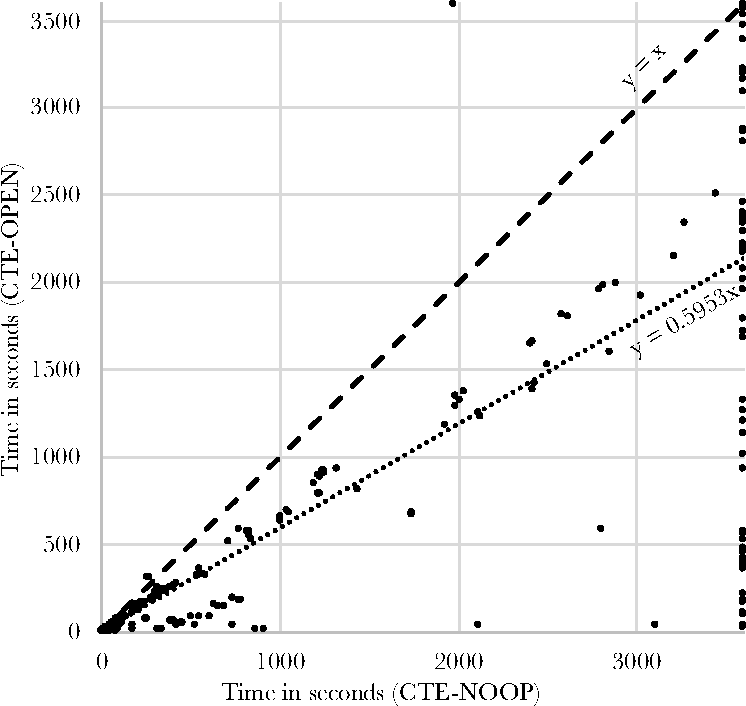
\includegraphics[width=.48\textwidth]{figures/time-plansat-open-noop3} \end{center}
\caption{Temps de décision (EFA/OPEN vs NOOP).}
\label{fig:plansat-noop}
\end{figure}

Nous avons testé la résolution de ces benchmarks avec nos nouveaux codages CTE-EFA et CTE-OPEN ainsi qu'avec le codage de l'état de l'art CTE-NOOP. Nous les avons comparés deux par deux en considérant le temps nécessaire pour prouver l'existence d'un plan (temps de décision, Figure~\ref{fig:plansat-noop}) et le temps global nécessaire pour obtenir un plan (temps d'extraction, Figure~\ref{fig:planextract-noop}). L'étape \enquote{décision} consiste à lancer de façon incrémentale le solveur QBF sur un CTE de profondeur croissante jusqu'à ce que le solveur retourne vrai ou atteigne la borne supérieure (nombre total de fluents). L'étape \enquote{extraction} consiste en un lancement du solveur par n\oe ud de l'arbre afin de récupérer le plan. Chaque test avait 60 minutes\footnote{L'étape d'instanciation des actions n'est pas incluse dans le temps écoulé.} de timeout pour la recherche du plan et 60 minutes pour son extraction.
Les résultats complets sont disponibles en ligne dans un fichier Excel\footnote{\url{https://www.irit.fr/~Frederic.Maris/documents/coplas2018/results.xls}}.

\begin{table*}
\centering
\begin{small}
\begin{tabular}{@{}lccccc@{}}
\toprule
Codage & Problèmes résolus & Temps de décision & Littéraux & Clauses & T/N \\ \midrule
CTE-NOOP & 412 sur 2112 (20\%) & 0\% & 0\% & 0\% & 30\% \\
CTE-EFA & 463 sur 2112 (22\%) & -55\% & -26\% & +15\% & 47\%  \\
CTE-OPEN & 445 sur 2112 (21\%) & -41\% & -2\% & -28\% & 17\% \\ \bottomrule
\\
\end{tabular}
\end{small}
\caption{Comparaison des codages présentés dans 65 domaines STRIPS des IPC 1 à 8 (sauf IPC 7) avec un total de 2112 problèmes. Le temps de décision, le nombre de littéraux, le nombre de clauses et le rapport transitions-sur-n\oe uds sont des moyennes. Transitions-sur-n\oe uds est le rapport moyen du nombre de contraintes basées sur des transitions divisé par le nombre de contraintes basées sur des n\oe uds (cf. Hypothèse 2, section Discussion ci-après).}
\label{fig:comparative}
\end{table*}

Les résultats montrent que nos codages CTE-EFA et CTE-OPEN sont plus efficaces que CTE-NOOP tant pour décider de l'existence d'un plan que pour l'extraire. CTE-EFA d'un facteur de 2,1 (1/0,4843) et CTE-OPEN d'un facteur de 1,7 (1/0,5953).  De plus, la comparaison entre CTE-EFA et CTE-OPEN (Figure~\ref{fig:plansat}, Figure~\ref{fig:planextract}) montre que CTE-EFA surpasse CTE-OPEN d'un facteur de 1,4 (1/0,7266). La Table~\ref{fig:comparative} donne un résumé des résultats sur les problèmes de référence.


% On IPC\_5/rovers/Propositional/Strips, the number of clauses and literals are very similar between NOOP and EFA. That said, EFA performs 46\% faster (in average).
% The correlation between the number of clauses and the performance gap between NOOP and EFA is not obvious. On average, NOOP encodings have 59\% more clauses than their EFA counterpart with the same number of literals
% OPEN encodings have the same number of clauses than NOOP but contain 20\% more literals.
%

Contrairement aux codages plats, le gain sur CTE-NOOP ne peut pas s'expliquer par une différence sur le nombre d'alternance des quantificateurs car la profondeur est la même dans les trois encodages. Cependant, la façon dont les actions sont représentées dans ces encodages pourrait expliquer cette différence.


\begin{figure}[ht!] \centering
\begin{center} 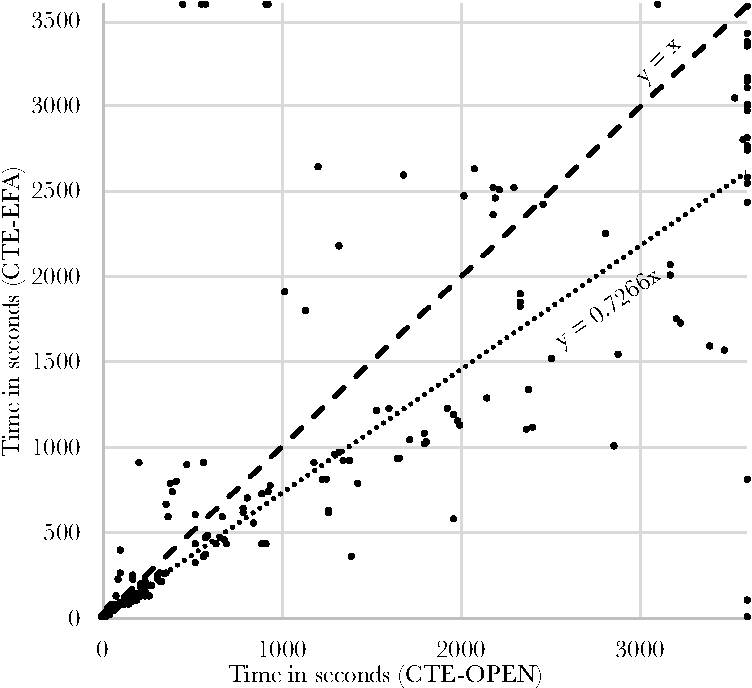
\includegraphics[width=.48\textwidth]{figures/time-plansat-efa-open3} \end{center}
\caption{Temps de décision (EFA vs OPEN).}
\label{fig:plansat}
\end{figure}

\begin{figure}[ht!] \centering
\begin{center} 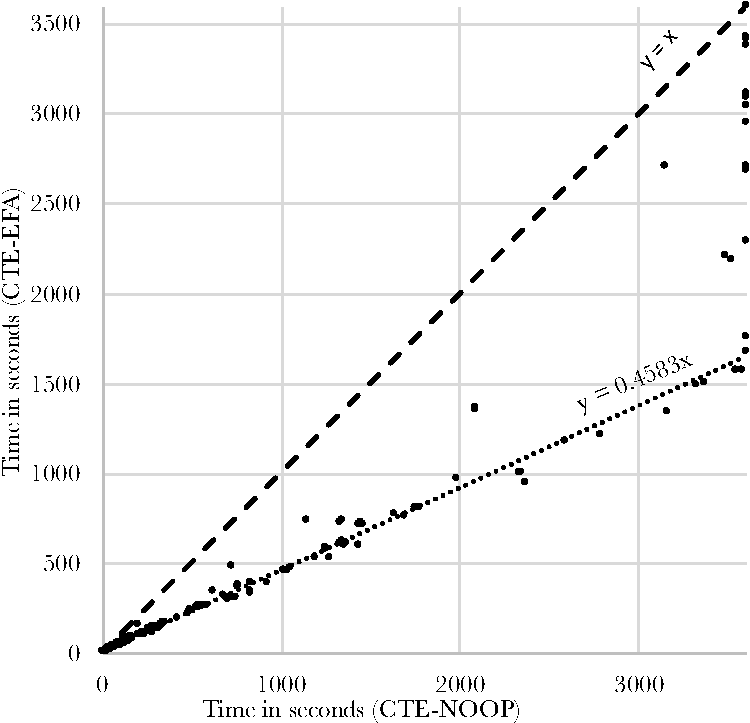
\includegraphics[width=.45\textwidth]{figures/time-extract-efa-noop3-good} %\end{center}
\hfill
%\begin{center} 
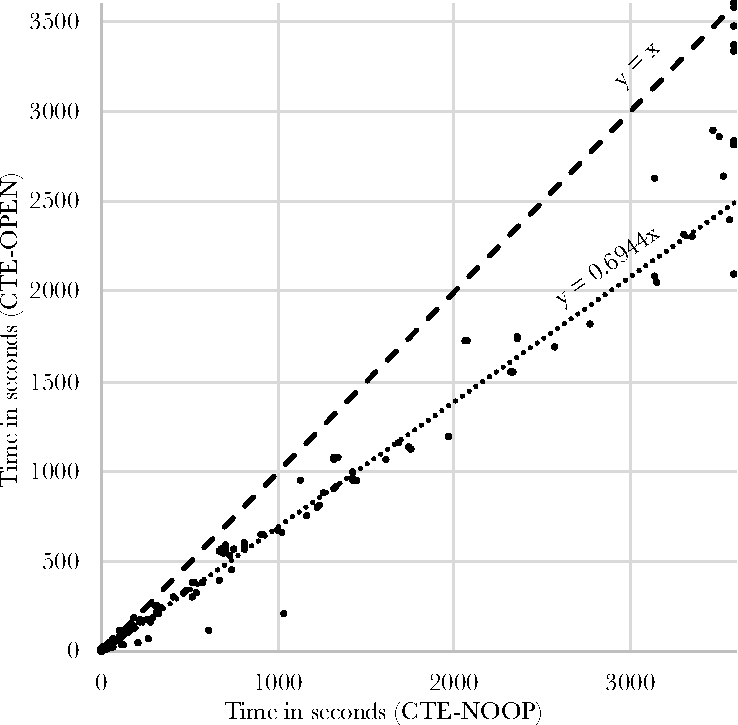
\includegraphics[width=.45\textwidth]{figures/time-extract-open-noop3} \end{center}
\caption{Temps d'extraction (EFA/OPEN vs NOOP).}
\label{fig:planextract-noop}
\end{figure}

\begin{figure}[ht!] \centering
\begin{center} 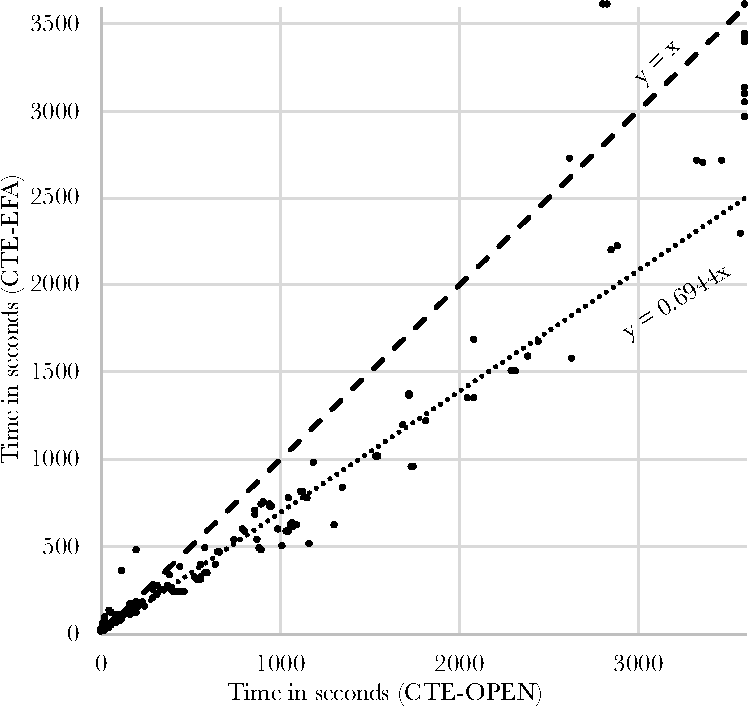
\includegraphics[width=.45\textwidth]{figures/time-extract-efa-open3-good} \end{center}
\caption{Temps d'extraction (EFA vs OPEN).}
\label{fig:planextract}
\end{figure}

\subsection{Discussion}

Pour tenter d'identifier les causes possibles de ces améliorations, nous avons proposé deux hypothèses, mises ensuite à l'épreuve avec nos tests:

\begin{description}
\item[Hypothèse 1] \enquote{Le gain de performance est corrélé à une diminution du nombre de clauses et/ou de littéraux à travers les encodages}. Bien que la taille du problème soit notoirement non-corrélée à sa difficulté dans SAT, nous nous sommes demandés si nous pourrions voir la même non-corrélation. Comme le montre la Table~\ref{fig:comparative}, nous n'observons aucune tendance claire: CTE-EFA tend à avoir un nombre de clauses légèrement plus élevé (+15\%) que CTE-NOOP bien qu'il ait moins de variables (-26\%). CTE-OPEN a le même nombre de littéraux et beaucoup moins de clauses que CTE-NOOP, mais avec un gain de performances inférieur (-41\%) à CTE-EFA (-55\%). Cette non-corrélation nous a conduit à rejeter cette hypothèse.
~\\

\item[Hypothèse 2] \enquote{Le gain de performance est dû à une différence dans le nombre de contraintes basées sur une transition par rapport au nombre de contraintes basées sur un n\oe ud}. Intuitivement, on peut penser qu'un ratio plus faible de contraintes basées sur les transitions sur les contraintes basées sur les n\oe uds faciliterait le processus de résolution: dans les contraintes basées sur les n\oe uds, une clause a le même contexte\footnote {Contexte et expansion sont définis dans \cite{DBLP:conf/ecai/CashmoreFG12}. Intuitivement, l'expansion est un arbre représentant la formule QBF et un contexte est une feuille dans cet arbre.} à travers l'extension QBF entière. Dans les contraintes de branche, la clause correspondante a des contextes différents selon la branche sélectionnée. L'idée est que les clauses basées sur différents contextes ralentissent le solveur. Comme le montre la Table~\ref{fig:comparative}, cette hypothèse ne semble pas pouvoir être étayée sur le plan expérimental: bien que CTE-OPEN montre un rapport transitions-sur-n\oe uds plus faible, il n'aboutit pas au meilleur gain de performance. Au contraire, le rapport CTE-EFA est plus faible, bien qu'il soit le plus efficace par rapport à CTE-NOOP. Nous avons donc aussi rejeté cette explication car nous n'avons noté aucune corrélation la soutenant, malgré une légère tendance où la diminution du temps et le nombre de clauses semblaient corrélées.
\end{description}

Aucune de nos deux hypothèses ne semblant donc être valable, la question de l'explication des gains de performance apportés par nos codages reste ouverte et sera l'objet de nos prochaines recherches.


\begin{figure}[ht!] \centering
\begin{center} 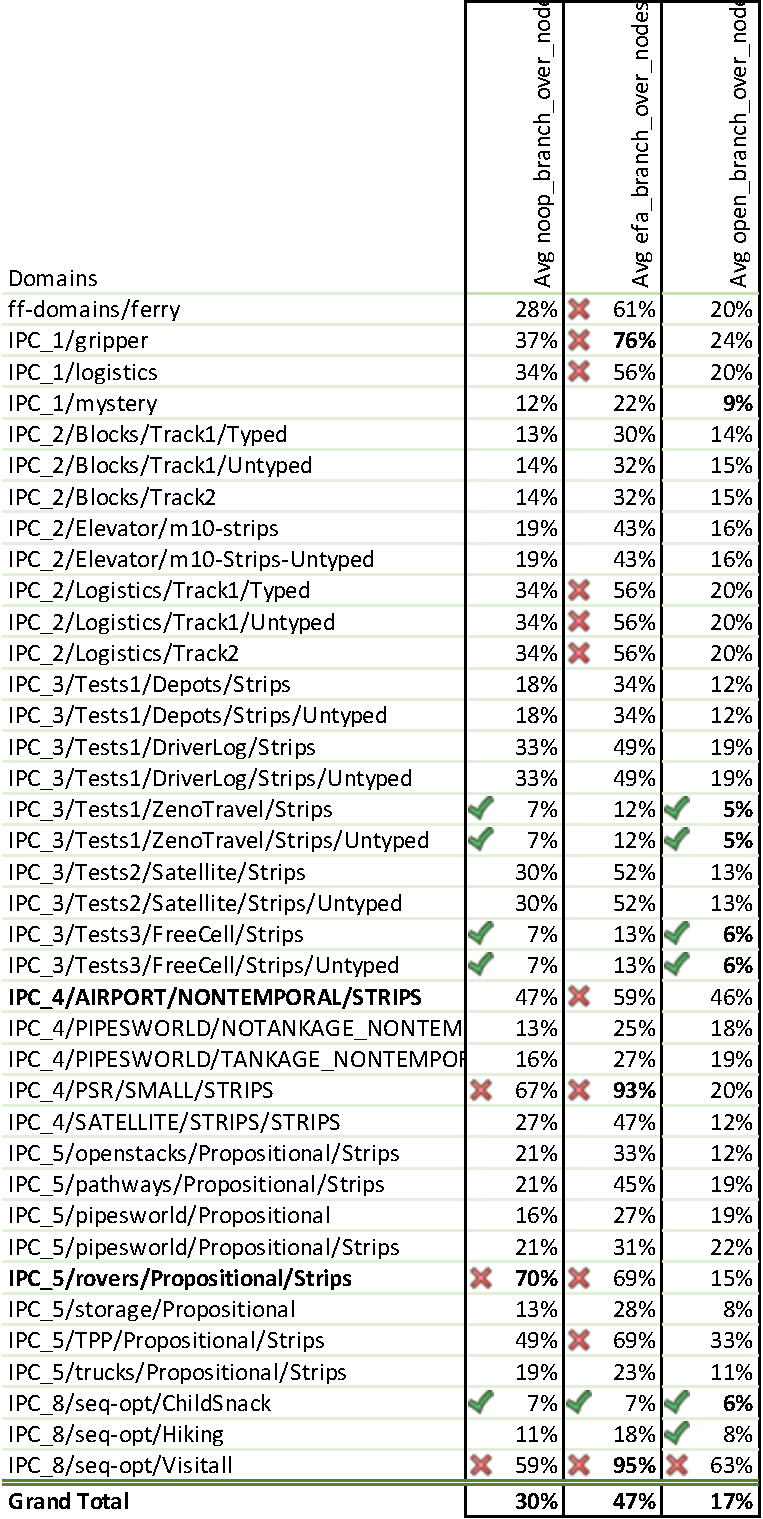
\includegraphics[width=.75\textwidth]{figures/experiment-branch_vs_nodes-crop.pdf} \end{center}
\caption{Rapport moyen B/N.}
\label{fig:tab-exp-branch-vs-nodes}
\end{figure}

\begin{figure}[ht!] \centering
\begin{center} 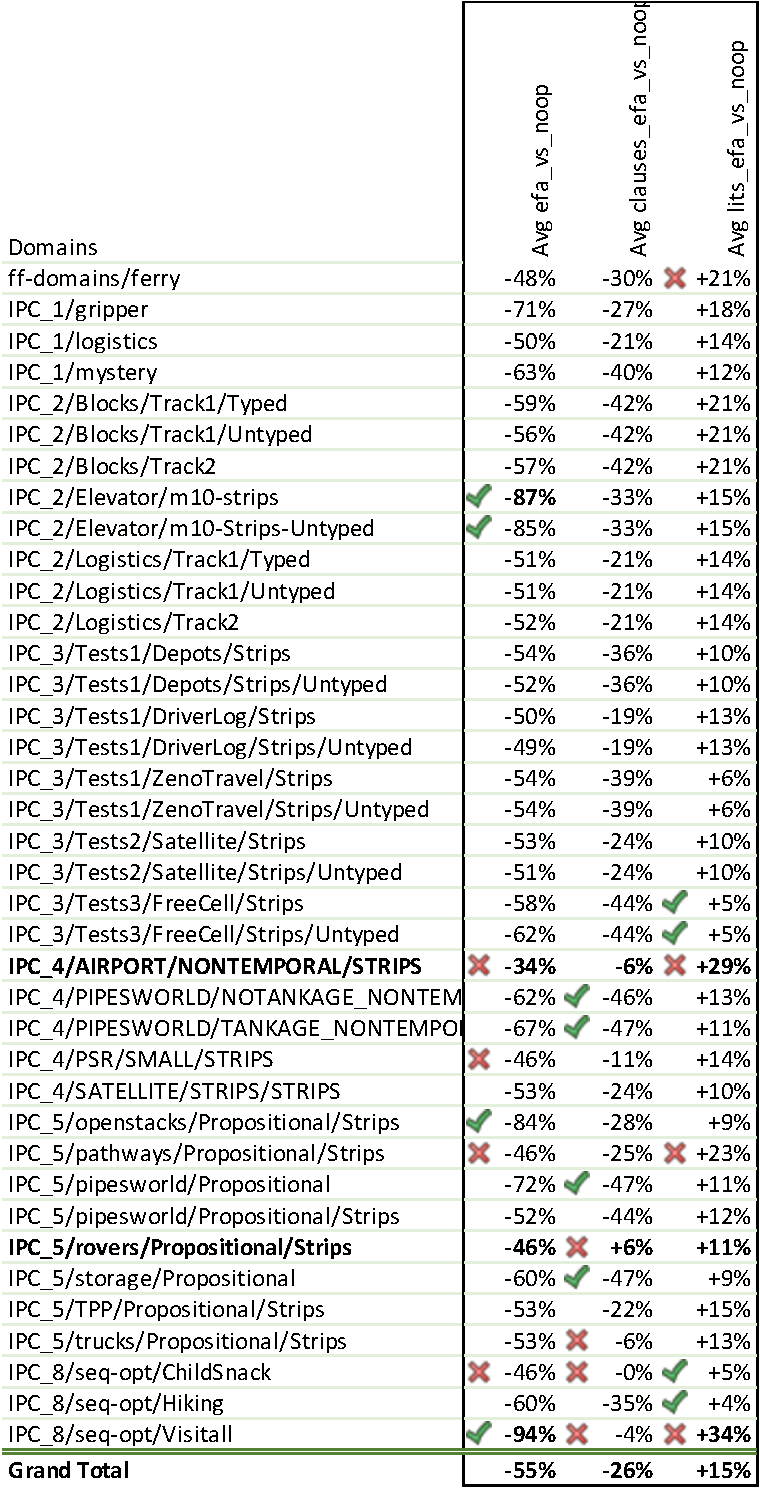
\includegraphics[width=.75\textwidth]{figures/experiment-efa_vs_noop-crop.pdf} \end{center}
\caption{Rapport moyen des performances CTE-EFA/CTE-NOOP.}
\label{fig:tab-exp-efa-vs-noop}
\end{figure}

\begin{figure}[ht!] \centering
\begin{center} 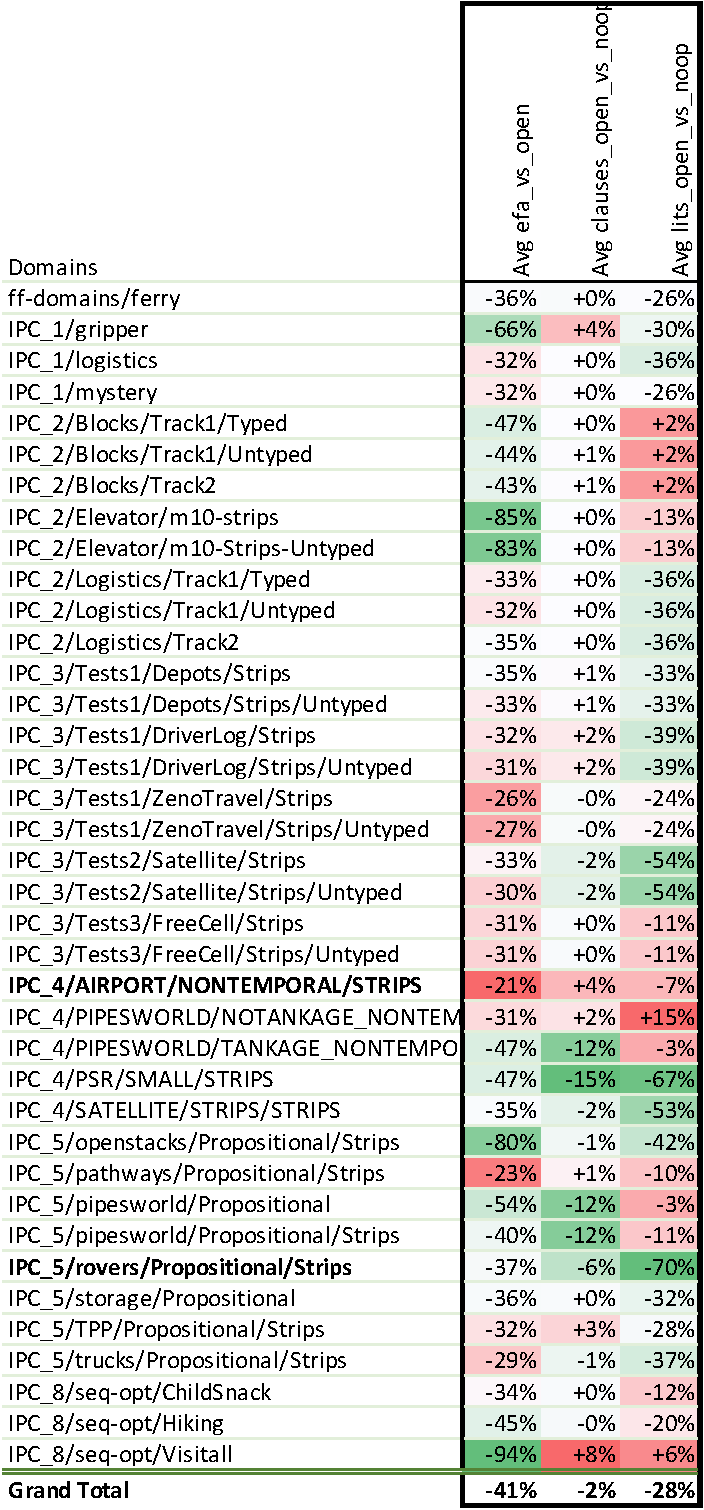
\includegraphics[width=.75\textwidth]{figures/experiment-efa_vs_open-crop.pdf} \end{center}
\caption{Rapport moyen des performances CTE-EFA/CTE-OPEN.}
\label{fig:tab-exp-efa-vs-open}
\end{figure}

%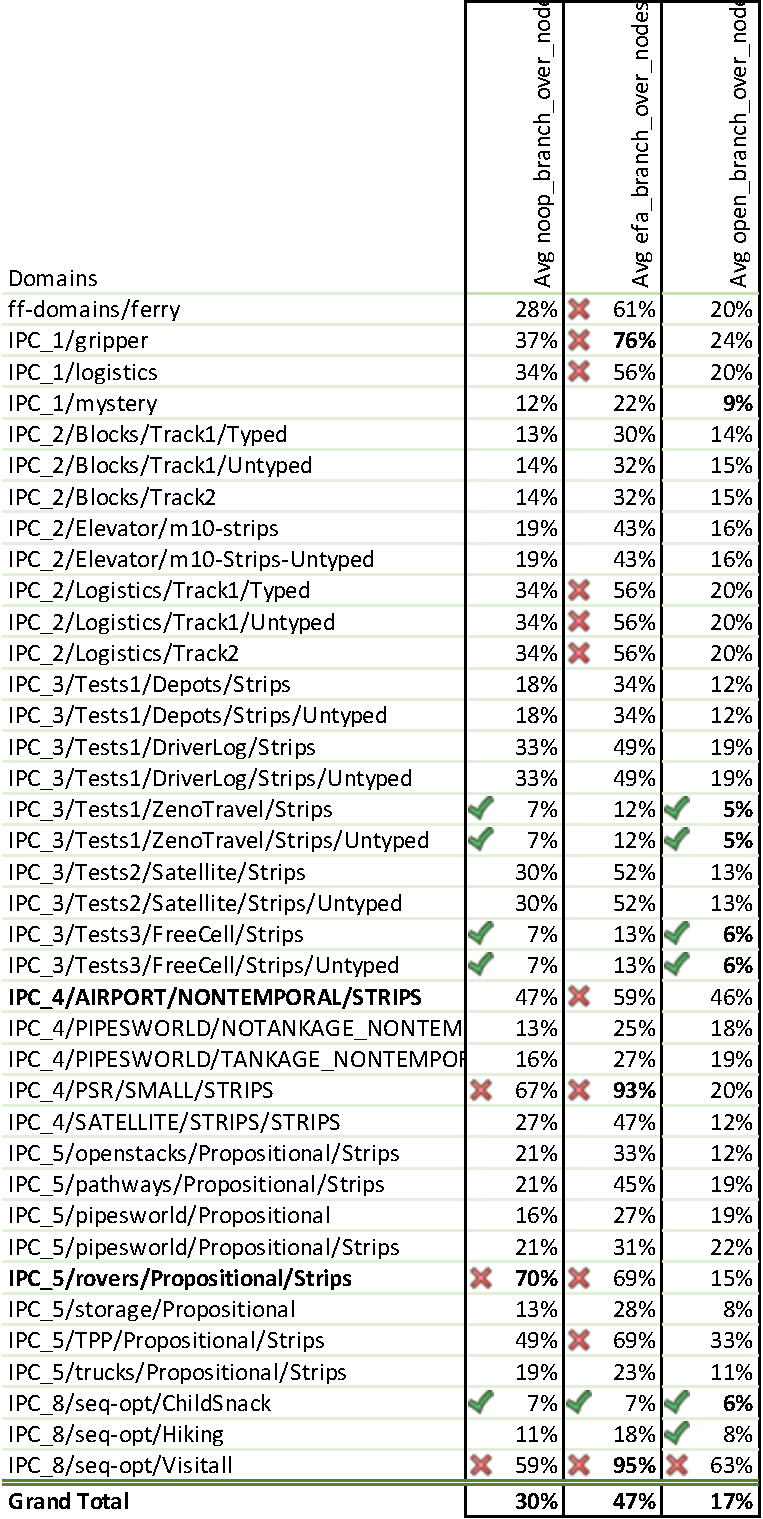
\includegraphics[width=0.5\textwidth]{figures/experiment-branch_vs_nodes-crop.pdf}

%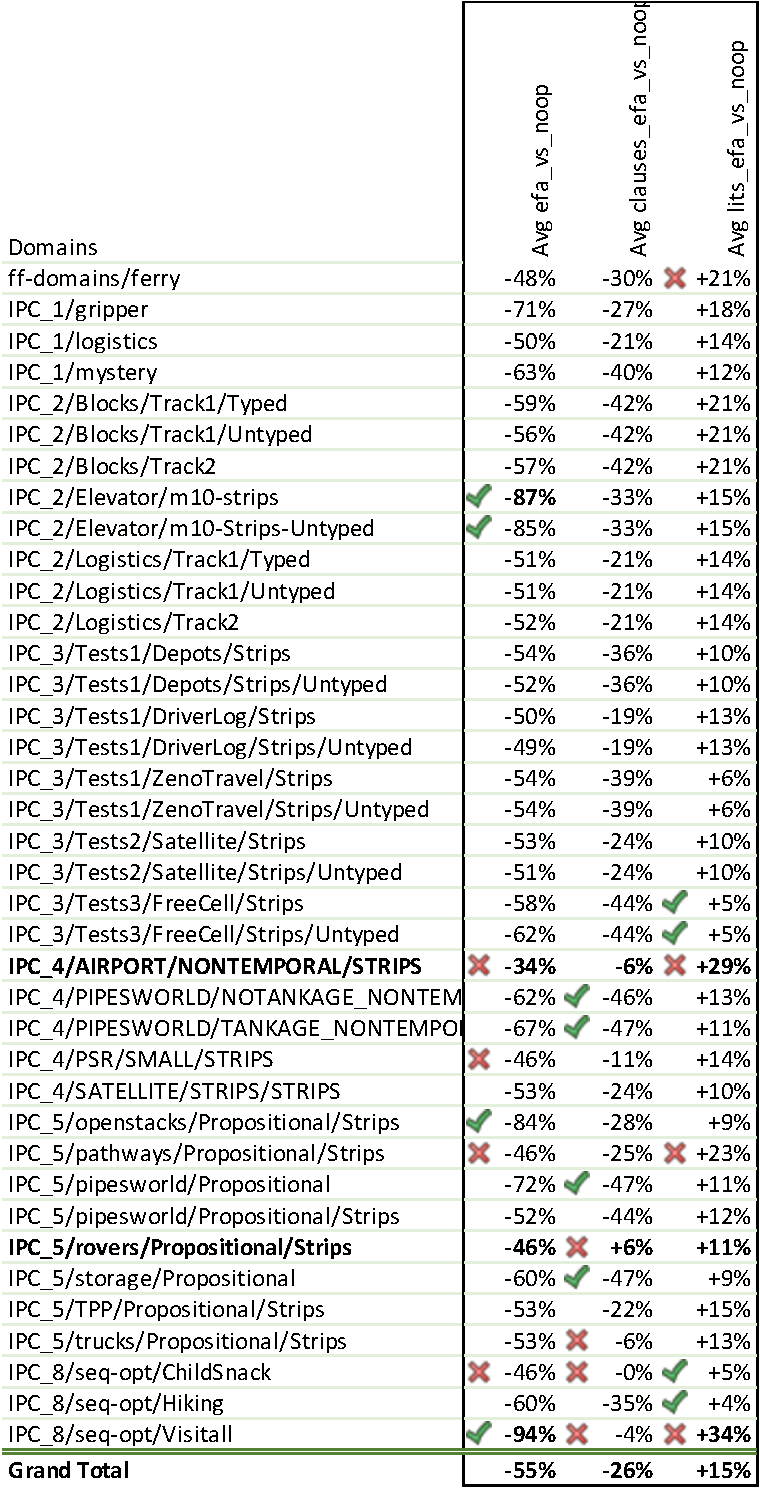
\includegraphics[scale=0.95]{figures/experiment-efa_vs_noop-crop.pdf}

%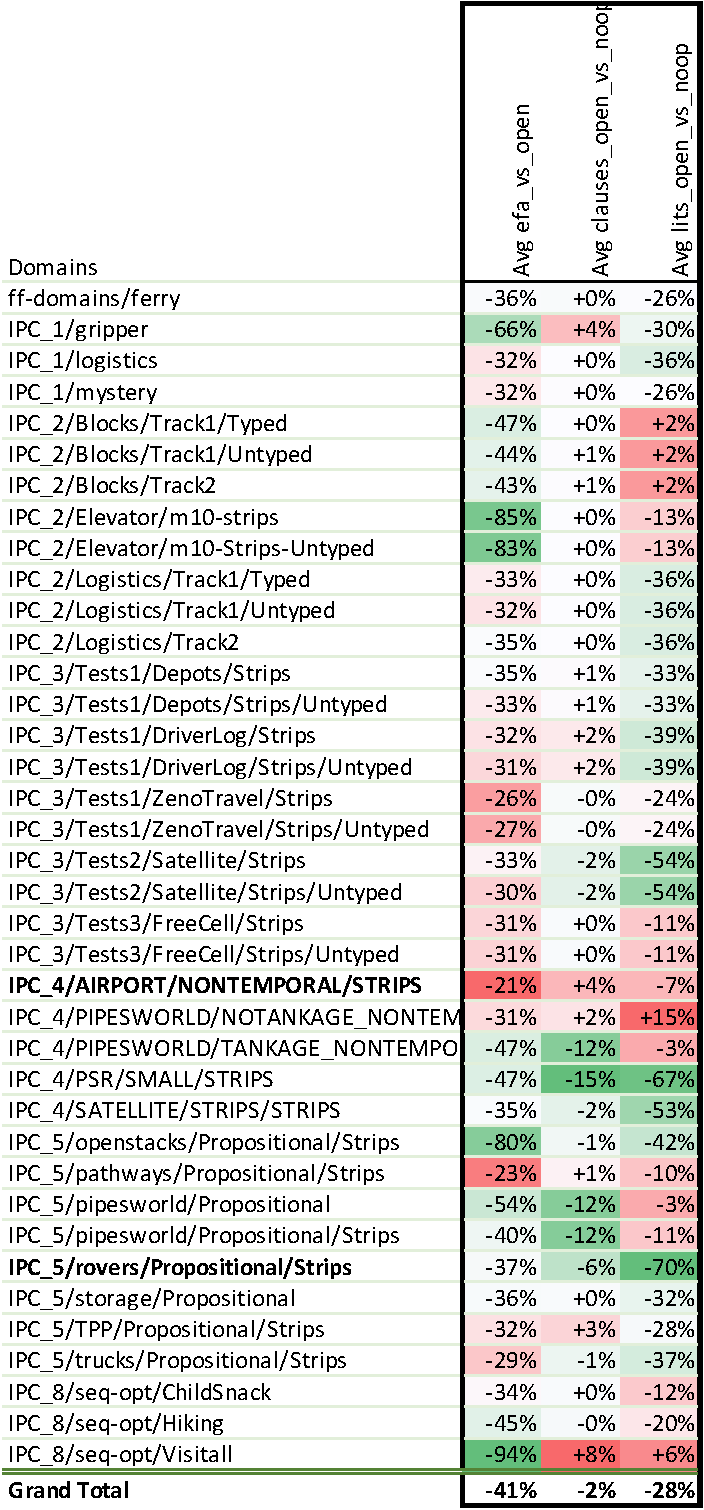
\includegraphics{figures/experiment-efa_vs_open-crop.pdf}


%%%%%%%%%%%%%%%%%%%%%%%%%%%%%%%%%%%%%%%%%%%%%%%%%%%%%%%%%%%%
% TESTS : PLANIFICATION SMT
%%%%%%%%%%%%%%%%%%%%%%%%%%%%%
%\subsection{Planification temporelle avec SMT}